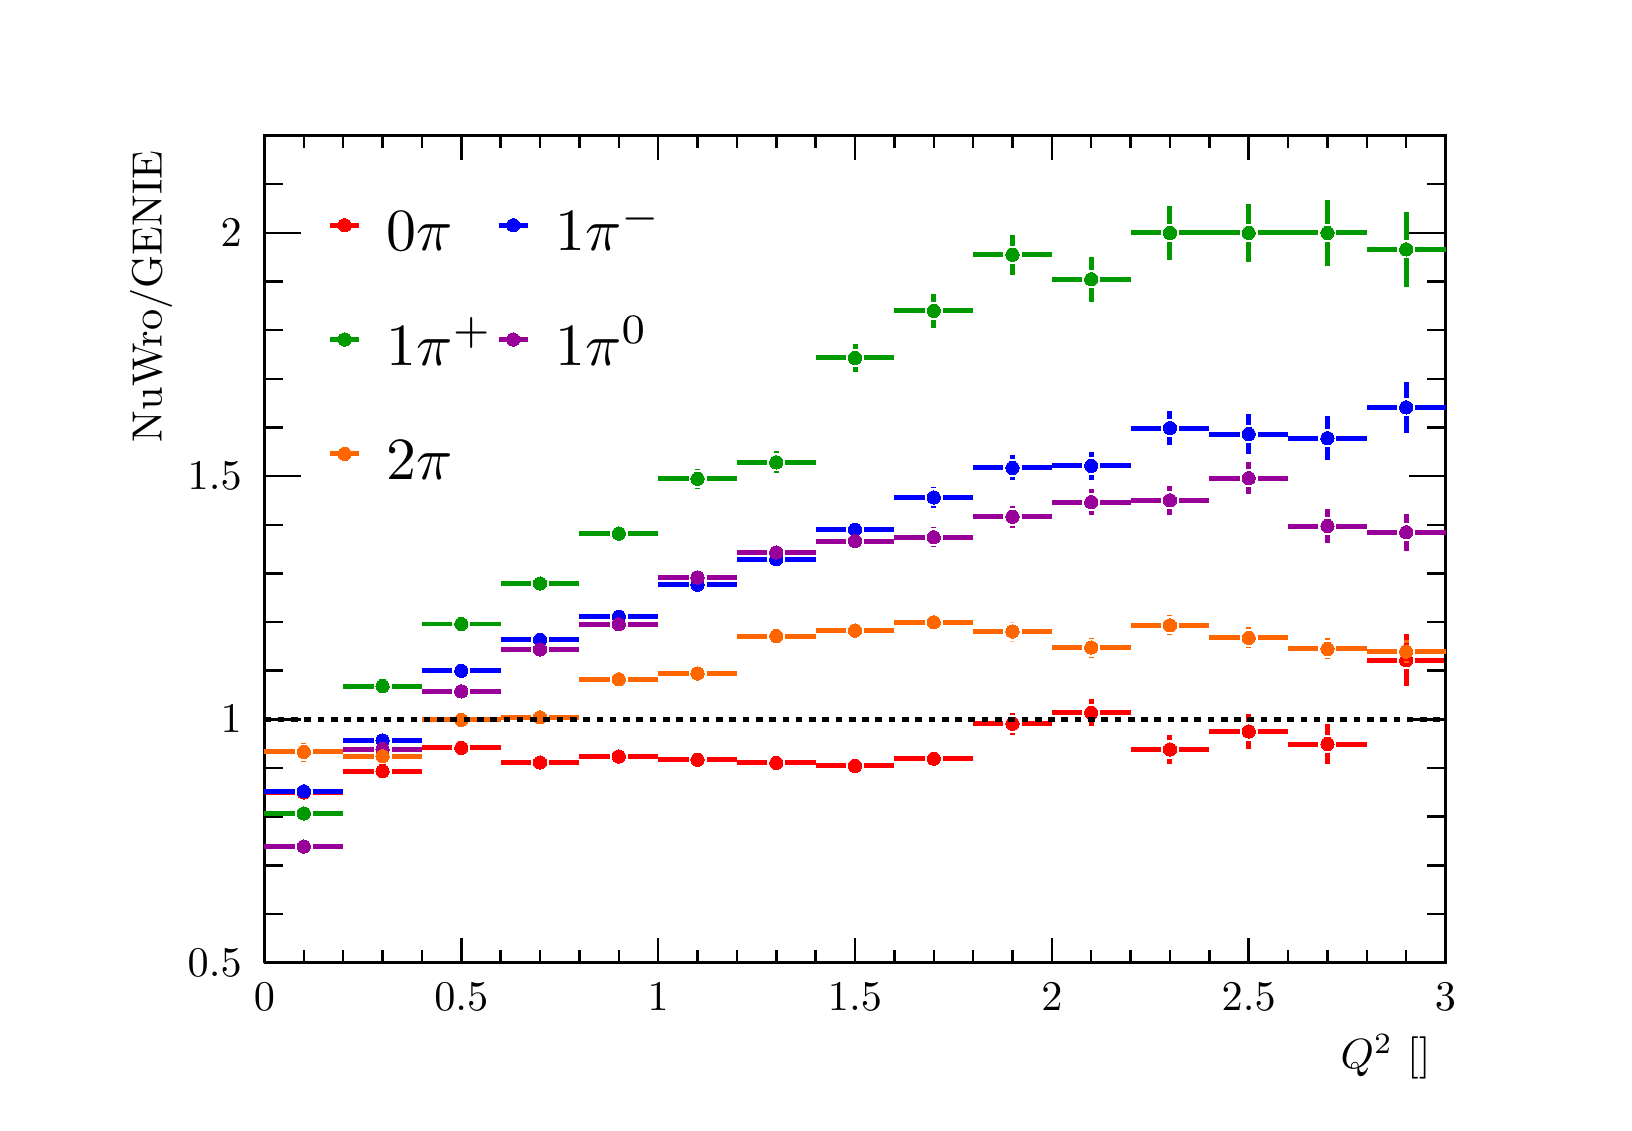
\begin{tikzpicture}
\pgfdeclareplotmark{cross} {
\pgfpathmoveto{\pgfpoint{-0.3\pgfplotmarksize}{\pgfplotmarksize}}
\pgfpathlineto{\pgfpoint{+0.3\pgfplotmarksize}{\pgfplotmarksize}}
\pgfpathlineto{\pgfpoint{+0.3\pgfplotmarksize}{0.3\pgfplotmarksize}}
\pgfpathlineto{\pgfpoint{+1\pgfplotmarksize}{0.3\pgfplotmarksize}}
\pgfpathlineto{\pgfpoint{+1\pgfplotmarksize}{-0.3\pgfplotmarksize}}
\pgfpathlineto{\pgfpoint{+0.3\pgfplotmarksize}{-0.3\pgfplotmarksize}}
\pgfpathlineto{\pgfpoint{+0.3\pgfplotmarksize}{-1.\pgfplotmarksize}}
\pgfpathlineto{\pgfpoint{-0.3\pgfplotmarksize}{-1.\pgfplotmarksize}}
\pgfpathlineto{\pgfpoint{-0.3\pgfplotmarksize}{-0.3\pgfplotmarksize}}
\pgfpathlineto{\pgfpoint{-1.\pgfplotmarksize}{-0.3\pgfplotmarksize}}
\pgfpathlineto{\pgfpoint{-1.\pgfplotmarksize}{0.3\pgfplotmarksize}}
\pgfpathlineto{\pgfpoint{-0.3\pgfplotmarksize}{0.3\pgfplotmarksize}}
\pgfpathclose
\pgfusepathqstroke
}
\pgfdeclareplotmark{cross*} {
\pgfpathmoveto{\pgfpoint{-0.3\pgfplotmarksize}{\pgfplotmarksize}}
\pgfpathlineto{\pgfpoint{+0.3\pgfplotmarksize}{\pgfplotmarksize}}
\pgfpathlineto{\pgfpoint{+0.3\pgfplotmarksize}{0.3\pgfplotmarksize}}
\pgfpathlineto{\pgfpoint{+1\pgfplotmarksize}{0.3\pgfplotmarksize}}
\pgfpathlineto{\pgfpoint{+1\pgfplotmarksize}{-0.3\pgfplotmarksize}}
\pgfpathlineto{\pgfpoint{+0.3\pgfplotmarksize}{-0.3\pgfplotmarksize}}
\pgfpathlineto{\pgfpoint{+0.3\pgfplotmarksize}{-1.\pgfplotmarksize}}
\pgfpathlineto{\pgfpoint{-0.3\pgfplotmarksize}{-1.\pgfplotmarksize}}
\pgfpathlineto{\pgfpoint{-0.3\pgfplotmarksize}{-0.3\pgfplotmarksize}}
\pgfpathlineto{\pgfpoint{-1.\pgfplotmarksize}{-0.3\pgfplotmarksize}}
\pgfpathlineto{\pgfpoint{-1.\pgfplotmarksize}{0.3\pgfplotmarksize}}
\pgfpathlineto{\pgfpoint{-0.3\pgfplotmarksize}{0.3\pgfplotmarksize}}
\pgfpathclose
\pgfusepathqfillstroke
}
\pgfdeclareplotmark{newstar} {
\pgfpathmoveto{\pgfqpoint{0pt}{\pgfplotmarksize}}
\pgfpathlineto{\pgfqpointpolar{44}{0.5\pgfplotmarksize}}
\pgfpathlineto{\pgfqpointpolar{18}{\pgfplotmarksize}}
\pgfpathlineto{\pgfqpointpolar{-20}{0.5\pgfplotmarksize}}
\pgfpathlineto{\pgfqpointpolar{-54}{\pgfplotmarksize}}
\pgfpathlineto{\pgfqpointpolar{-90}{0.5\pgfplotmarksize}}
\pgfpathlineto{\pgfqpointpolar{234}{\pgfplotmarksize}}
\pgfpathlineto{\pgfqpointpolar{198}{0.5\pgfplotmarksize}}
\pgfpathlineto{\pgfqpointpolar{162}{\pgfplotmarksize}}
\pgfpathlineto{\pgfqpointpolar{134}{0.5\pgfplotmarksize}}
\pgfpathclose
\pgfusepathqstroke
}
\pgfdeclareplotmark{newstar*} {
\pgfpathmoveto{\pgfqpoint{0pt}{\pgfplotmarksize}}
\pgfpathlineto{\pgfqpointpolar{44}{0.5\pgfplotmarksize}}
\pgfpathlineto{\pgfqpointpolar{18}{\pgfplotmarksize}}
\pgfpathlineto{\pgfqpointpolar{-20}{0.5\pgfplotmarksize}}
\pgfpathlineto{\pgfqpointpolar{-54}{\pgfplotmarksize}}
\pgfpathlineto{\pgfqpointpolar{-90}{0.5\pgfplotmarksize}}
\pgfpathlineto{\pgfqpointpolar{234}{\pgfplotmarksize}}
\pgfpathlineto{\pgfqpointpolar{198}{0.5\pgfplotmarksize}}
\pgfpathlineto{\pgfqpointpolar{162}{\pgfplotmarksize}}
\pgfpathlineto{\pgfqpointpolar{134}{0.5\pgfplotmarksize}}
\pgfpathclose
\pgfusepathqfillstroke
}
\definecolor{c}{rgb}{1,1,1};
\draw [color=c, fill=c] (0,0) rectangle (20,13.639);
\draw [color=c, fill=c] (3,1.77307) rectangle (18,12.2751);
\definecolor{c}{rgb}{0,0,0};
\draw [c,line width=0.9] (3,1.77307) -- (3,12.2751) -- (18,12.2751) -- (18,1.77307) -- (3,1.77307);
\definecolor{c}{rgb}{1,1,1};
\draw [color=c, fill=c] (3,1.77307) rectangle (18,12.2751);
\definecolor{c}{rgb}{0,0,0};
\draw [c,line width=0.9] (3,1.77307) -- (3,12.2751) -- (18,12.2751) -- (18,1.77307) -- (3,1.77307);
\definecolor{c}{rgb}{1,0,0};
\draw [c,line width=1.8] (3,3.93291) -- (3.38539,3.93291);
\draw [c,line width=1.8] (3.61461,3.93291) -- (4,3.93291);
\foreach \P in {(3.5,3.93291)}{\draw[mark options={color=c,fill=c},mark size=2.402402pt, line width=0.000000pt, mark=*] plot coordinates {\P};}
\draw [c,line width=1.8] (4,4.2042) -- (4.38539,4.2042);
\draw [c,line width=1.8] (4.61461,4.2042) -- (5,4.2042);
\foreach \P in {(4.5,4.2042)}{\draw[mark options={color=c,fill=c},mark size=2.402402pt, line width=0.000000pt, mark=*] plot coordinates {\P};}
\draw [c,line width=1.8] (5,4.50007) -- (5.38539,4.50007);
\draw [c,line width=1.8] (5.61461,4.50007) -- (6,4.50007);
\foreach \P in {(5.5,4.50007)}{\draw[mark options={color=c,fill=c},mark size=2.402402pt, line width=0.000000pt, mark=*] plot coordinates {\P};}
\draw [c,line width=1.8] (6,4.31341) -- (6.38539,4.31341);
\draw [c,line width=1.8] (6.61461,4.31341) -- (7,4.31341);
\foreach \P in {(6.5,4.31341)}{\draw[mark options={color=c,fill=c},mark size=2.402402pt, line width=0.000000pt, mark=*] plot coordinates {\P};}
\draw [c,line width=1.8] (7,4.38948) -- (7.38539,4.38948);
\draw [c,line width=1.8] (7.61461,4.38948) -- (8,4.38948);
\foreach \P in {(7.5,4.38948)}{\draw[mark options={color=c,fill=c},mark size=2.402402pt, line width=0.000000pt, mark=*] plot coordinates {\P};}
\draw [c,line width=1.8] (8,4.34832) -- (8.38539,4.34832);
\draw [c,line width=1.8] (8.61461,4.34832) -- (9,4.34832);
\foreach \P in {(8.5,4.34832)}{\draw[mark options={color=c,fill=c},mark size=2.402402pt, line width=0.000000pt, mark=*] plot coordinates {\P};}
\draw [c,line width=1.8] (9,4.3085) -- (9.38539,4.3085);
\draw [c,line width=1.8] (9.61461,4.3085) -- (10,4.3085);
\foreach \P in {(9.5,4.3085)}{\draw[mark options={color=c,fill=c},mark size=2.402402pt, line width=0.000000pt, mark=*] plot coordinates {\P};}
\draw [c,line width=1.8] (10,4.27069) -- (10.3854,4.27069);
\draw [c,line width=1.8] (10.6146,4.27069) -- (11,4.27069);
\foreach \P in {(10.5,4.27069)}{\draw[mark options={color=c,fill=c},mark size=2.402402pt, line width=0.000000pt, mark=*] plot coordinates {\P};}
\draw [c,line width=1.8] (11,4.3619) -- (11.3854,4.3619);
\draw [c,line width=1.8] (11.6146,4.3619) -- (12,4.3619);
\foreach \P in {(11.5,4.3619)}{\draw[mark options={color=c,fill=c},mark size=2.402402pt, line width=0.000000pt, mark=*] plot coordinates {\P};}
\draw [c,line width=1.8] (12.5,4.66464) -- (12.5,4.69177);
\draw [c,line width=1.8] (12.5,4.92099) -- (12.5,4.94812);
\draw [c,line width=1.8] (12,4.80638) -- (12.3854,4.80638);
\draw [c,line width=1.8] (12.6146,4.80638) -- (13,4.80638);
\foreach \P in {(12.5,4.80638)}{\draw[mark options={color=c,fill=c},mark size=2.402402pt, line width=0.000000pt, mark=*] plot coordinates {\P};}
\draw [c,line width=1.8] (13.5,4.7751) -- (13.5,4.83015);
\draw [c,line width=1.8] (13.5,5.05937) -- (13.5,5.11442);
\draw [c,line width=1.8] (13,4.94476) -- (13.3854,4.94476);
\draw [c,line width=1.8] (13.6146,4.94476) -- (14,4.94476);
\foreach \P in {(13.5,4.94476)}{\draw[mark options={color=c,fill=c},mark size=2.402402pt, line width=0.000000pt, mark=*] plot coordinates {\P};}
\draw [c,line width=1.8] (14.5,4.28886) -- (14.5,4.36427);
\draw [c,line width=1.8] (14.5,4.5935) -- (14.5,4.66892);
\draw [c,line width=1.8] (14,4.47889) -- (14.3854,4.47889);
\draw [c,line width=1.8] (14.6146,4.47889) -- (15,4.47889);
\foreach \P in {(14.5,4.47889)}{\draw[mark options={color=c,fill=c},mark size=2.402402pt, line width=0.000000pt, mark=*] plot coordinates {\P};}
\draw [c,line width=1.8] (15.5,4.4814) -- (15.5,4.59289);
\draw [c,line width=1.8] (15.5,4.82212) -- (15.5,4.93361);
\draw [c,line width=1.8] (15,4.70751) -- (15.3854,4.70751);
\draw [c,line width=1.8] (15.6146,4.70751) -- (16,4.70751);
\foreach \P in {(15.5,4.70751)}{\draw[mark options={color=c,fill=c},mark size=2.402402pt, line width=0.000000pt, mark=*] plot coordinates {\P};}
\draw [c,line width=1.8] (16.5,4.28844) -- (16.5,4.43366);
\draw [c,line width=1.8] (16.5,4.66289) -- (16.5,4.8081);
\draw [c,line width=1.8] (16,4.54827) -- (16.3854,4.54827);
\draw [c,line width=1.8] (16.6146,4.54827) -- (17,4.54827);
\foreach \P in {(16.5,4.54827)}{\draw[mark options={color=c,fill=c},mark size=2.402402pt, line width=0.000000pt, mark=*] plot coordinates {\P};}
\draw [c,line width=1.8] (17.5,5.28277) -- (17.5,5.49737);
\draw [c,line width=1.8] (17.5,5.7266) -- (17.5,5.9412);
\draw [c,line width=1.8] (17,5.61199) -- (17.3854,5.61199);
\draw [c,line width=1.8] (17.6146,5.61199) -- (18,5.61199);
\foreach \P in {(17.5,5.61199)}{\draw[mark options={color=c,fill=c},mark size=2.402402pt, line width=0.000000pt, mark=*] plot coordinates {\P};}
\definecolor{c}{rgb}{0,0,0};
\draw [c,line width=0.9] (3,1.77307) -- (18,1.77307);
\draw [c,line width=0.9] (3,2.07994) -- (3,1.77307);
\draw [c,line width=0.9] (3.5,1.9265) -- (3.5,1.77307);
\draw [c,line width=0.9] (4,1.9265) -- (4,1.77307);
\draw [c,line width=0.9] (4.5,1.9265) -- (4.5,1.77307);
\draw [c,line width=0.9] (5,1.9265) -- (5,1.77307);
\draw [c,line width=0.9] (5.5,2.07994) -- (5.5,1.77307);
\draw [c,line width=0.9] (6,1.9265) -- (6,1.77307);
\draw [c,line width=0.9] (6.5,1.9265) -- (6.5,1.77307);
\draw [c,line width=0.9] (7,1.9265) -- (7,1.77307);
\draw [c,line width=0.9] (7.5,1.9265) -- (7.5,1.77307);
\draw [c,line width=0.9] (8,2.07994) -- (8,1.77307);
\draw [c,line width=0.9] (8.5,1.9265) -- (8.5,1.77307);
\draw [c,line width=0.9] (9,1.9265) -- (9,1.77307);
\draw [c,line width=0.9] (9.5,1.9265) -- (9.5,1.77307);
\draw [c,line width=0.9] (10,1.9265) -- (10,1.77307);
\draw [c,line width=0.9] (10.5,2.07994) -- (10.5,1.77307);
\draw [c,line width=0.9] (11,1.9265) -- (11,1.77307);
\draw [c,line width=0.9] (11.5,1.9265) -- (11.5,1.77307);
\draw [c,line width=0.9] (12,1.9265) -- (12,1.77307);
\draw [c,line width=0.9] (12.5,1.9265) -- (12.5,1.77307);
\draw [c,line width=0.9] (13,2.07994) -- (13,1.77307);
\draw [c,line width=0.9] (13.5,1.9265) -- (13.5,1.77307);
\draw [c,line width=0.9] (14,1.9265) -- (14,1.77307);
\draw [c,line width=0.9] (14.5,1.9265) -- (14.5,1.77307);
\draw [c,line width=0.9] (15,1.9265) -- (15,1.77307);
\draw [c,line width=0.9] (15.5,2.07994) -- (15.5,1.77307);
\draw [c,line width=0.9] (16,1.9265) -- (16,1.77307);
\draw [c,line width=0.9] (16.5,1.9265) -- (16.5,1.77307);
\draw [c,line width=0.9] (17,1.9265) -- (17,1.77307);
\draw [c,line width=0.9] (17.5,1.9265) -- (17.5,1.77307);
\draw [c,line width=0.9] (18,2.07994) -- (18,1.77307);
\draw [c,line width=0.9] (18,2.07994) -- (18,1.77307);
\draw [anchor=base] (3,1.15931) node[scale=1.52731, color=c, rotate=0]{0};
\draw [anchor=base] (5.5,1.15931) node[scale=1.52731, color=c, rotate=0]{0.5};
\draw [anchor=base] (8,1.15931) node[scale=1.52731, color=c, rotate=0]{1};
\draw [anchor=base] (10.5,1.15931) node[scale=1.52731, color=c, rotate=0]{1.5};
\draw [anchor=base] (13,1.15931) node[scale=1.52731, color=c, rotate=0]{2};
\draw [anchor=base] (15.5,1.15931) node[scale=1.52731, color=c, rotate=0]{2.5};
\draw [anchor=base] (18,1.15931) node[scale=1.52731, color=c, rotate=0]{3};
\draw [anchor= east] (18,0.572837) node[scale=1.52731, color=c, rotate=0]{$Q^{2}$ [\si{\GeV\squared}] };
\draw [c,line width=0.9] (3,12.2751) -- (18,12.2751);
\draw [c,line width=0.9] (3,11.9682) -- (3,12.2751);
\draw [c,line width=0.9] (3.5,12.1216) -- (3.5,12.2751);
\draw [c,line width=0.9] (4,12.1216) -- (4,12.2751);
\draw [c,line width=0.9] (4.5,12.1216) -- (4.5,12.2751);
\draw [c,line width=0.9] (5,12.1216) -- (5,12.2751);
\draw [c,line width=0.9] (5.5,11.9682) -- (5.5,12.2751);
\draw [c,line width=0.9] (6,12.1216) -- (6,12.2751);
\draw [c,line width=0.9] (6.5,12.1216) -- (6.5,12.2751);
\draw [c,line width=0.9] (7,12.1216) -- (7,12.2751);
\draw [c,line width=0.9] (7.5,12.1216) -- (7.5,12.2751);
\draw [c,line width=0.9] (8,11.9682) -- (8,12.2751);
\draw [c,line width=0.9] (8.5,12.1216) -- (8.5,12.2751);
\draw [c,line width=0.9] (9,12.1216) -- (9,12.2751);
\draw [c,line width=0.9] (9.5,12.1216) -- (9.5,12.2751);
\draw [c,line width=0.9] (10,12.1216) -- (10,12.2751);
\draw [c,line width=0.9] (10.5,11.9682) -- (10.5,12.2751);
\draw [c,line width=0.9] (11,12.1216) -- (11,12.2751);
\draw [c,line width=0.9] (11.5,12.1216) -- (11.5,12.2751);
\draw [c,line width=0.9] (12,12.1216) -- (12,12.2751);
\draw [c,line width=0.9] (12.5,12.1216) -- (12.5,12.2751);
\draw [c,line width=0.9] (13,11.9682) -- (13,12.2751);
\draw [c,line width=0.9] (13.5,12.1216) -- (13.5,12.2751);
\draw [c,line width=0.9] (14,12.1216) -- (14,12.2751);
\draw [c,line width=0.9] (14.5,12.1216) -- (14.5,12.2751);
\draw [c,line width=0.9] (15,12.1216) -- (15,12.2751);
\draw [c,line width=0.9] (15.5,11.9682) -- (15.5,12.2751);
\draw [c,line width=0.9] (16,12.1216) -- (16,12.2751);
\draw [c,line width=0.9] (16.5,12.1216) -- (16.5,12.2751);
\draw [c,line width=0.9] (17,12.1216) -- (17,12.2751);
\draw [c,line width=0.9] (17.5,12.1216) -- (17.5,12.2751);
\draw [c,line width=0.9] (18,11.9682) -- (18,12.2751);
\draw [c,line width=0.9] (18,11.9682) -- (18,12.2751);
\draw [c,line width=0.9] (3,1.77307) -- (3,12.2751);
\draw [c,line width=0.9] (3.462,1.77307) -- (3,1.77307);
\draw [c,line width=0.9] (3.231,2.39083) -- (3,2.39083);
\draw [c,line width=0.9] (3.231,3.0086) -- (3,3.0086);
\draw [c,line width=0.9] (3.231,3.62636) -- (3,3.62636);
\draw [c,line width=0.9] (3.231,4.24413) -- (3,4.24413);
\draw [c,line width=0.9] (3.462,4.86189) -- (3,4.86189);
\draw [c,line width=0.9] (3.231,5.47966) -- (3,5.47966);
\draw [c,line width=0.9] (3.231,6.09742) -- (3,6.09742);
\draw [c,line width=0.9] (3.231,6.71519) -- (3,6.71519);
\draw [c,line width=0.9] (3.231,7.33295) -- (3,7.33295);
\draw [c,line width=0.9] (3.462,7.95072) -- (3,7.95072);
\draw [c,line width=0.9] (3.231,8.56848) -- (3,8.56848);
\draw [c,line width=0.9] (3.231,9.18625) -- (3,9.18625);
\draw [c,line width=0.9] (3.231,9.80401) -- (3,9.80401);
\draw [c,line width=0.9] (3.231,10.4218) -- (3,10.4218);
\draw [c,line width=0.9] (3.462,11.0395) -- (3,11.0395);
\draw [c,line width=0.9] (3.462,11.0395) -- (3,11.0395);
\draw [c,line width=0.9] (3.231,11.6573) -- (3,11.6573);
\draw [c,line width=0.9] (3.231,12.2751) -- (3,12.2751);
\draw [anchor= east] (2.9,1.77307) node[scale=1.52731, color=c, rotate=0]{0.5};
\draw [anchor= east] (2.9,4.86189) node[scale=1.52731, color=c, rotate=0]{1};
\draw [anchor= east] (2.9,7.95072) node[scale=1.52731, color=c, rotate=0]{1.5};
\draw [anchor= east] (2.9,11.0395) node[scale=1.52731, color=c, rotate=0]{2};
\draw [anchor= east] (1.56,12.2751) node[scale=1.52731, color=c, rotate=90]{ NuWro/GENIE};
\draw [c,line width=0.9] (18,1.77307) -- (18,12.2751);
\draw [c,line width=0.9] (17.538,1.77307) -- (18,1.77307);
\draw [c,line width=0.9] (17.769,2.39083) -- (18,2.39083);
\draw [c,line width=0.9] (17.769,3.0086) -- (18,3.0086);
\draw [c,line width=0.9] (17.769,3.62636) -- (18,3.62636);
\draw [c,line width=0.9] (17.769,4.24413) -- (18,4.24413);
\draw [c,line width=0.9] (17.538,4.86189) -- (18,4.86189);
\draw [c,line width=0.9] (17.769,5.47966) -- (18,5.47966);
\draw [c,line width=0.9] (17.769,6.09742) -- (18,6.09742);
\draw [c,line width=0.9] (17.769,6.71519) -- (18,6.71519);
\draw [c,line width=0.9] (17.769,7.33295) -- (18,7.33295);
\draw [c,line width=0.9] (17.538,7.95072) -- (18,7.95072);
\draw [c,line width=0.9] (17.769,8.56848) -- (18,8.56848);
\draw [c,line width=0.9] (17.769,9.18625) -- (18,9.18625);
\draw [c,line width=0.9] (17.769,9.80401) -- (18,9.80401);
\draw [c,line width=0.9] (17.769,10.4218) -- (18,10.4218);
\draw [c,line width=0.9] (17.538,11.0395) -- (18,11.0395);
\draw [c,line width=0.9] (17.538,11.0395) -- (18,11.0395);
\draw [c,line width=0.9] (17.769,11.6573) -- (18,11.6573);
\draw [c,line width=0.9] (17.769,12.2751) -- (18,12.2751);
\definecolor{c}{rgb}{0,0,1};
\draw [c,line width=1.8] (3,3.94771) -- (3.38539,3.94771);
\draw [c,line width=1.8] (3.61461,3.94771) -- (4,3.94771);
\foreach \P in {(3.5,3.94771)}{\draw[mark options={color=c,fill=c},mark size=2.402402pt, line width=0.000000pt, mark=*] plot coordinates {\P};}
\draw [c,line width=1.8] (4,4.59342) -- (4.38539,4.59342);
\draw [c,line width=1.8] (4.61461,4.59342) -- (5,4.59342);
\foreach \P in {(4.5,4.59342)}{\draw[mark options={color=c,fill=c},mark size=2.402402pt, line width=0.000000pt, mark=*] plot coordinates {\P};}
\draw [c,line width=1.8] (5,5.47872) -- (5.38539,5.47872);
\draw [c,line width=1.8] (5.61461,5.47872) -- (6,5.47872);
\foreach \P in {(5.5,5.47872)}{\draw[mark options={color=c,fill=c},mark size=2.402402pt, line width=0.000000pt, mark=*] plot coordinates {\P};}
\draw [c,line width=1.8] (6,5.87289) -- (6.38539,5.87289);
\draw [c,line width=1.8] (6.61461,5.87289) -- (7,5.87289);
\foreach \P in {(6.5,5.87289)}{\draw[mark options={color=c,fill=c},mark size=2.402402pt, line width=0.000000pt, mark=*] plot coordinates {\P};}
\draw [c,line width=1.8] (7,6.16572) -- (7.38539,6.16572);
\draw [c,line width=1.8] (7.61461,6.16572) -- (8,6.16572);
\foreach \P in {(7.5,6.16572)}{\draw[mark options={color=c,fill=c},mark size=2.402402pt, line width=0.000000pt, mark=*] plot coordinates {\P};}
\draw [c,line width=1.8] (8,6.57211) -- (8.38539,6.57211);
\draw [c,line width=1.8] (8.61461,6.57211) -- (9,6.57211);
\foreach \P in {(8.5,6.57211)}{\draw[mark options={color=c,fill=c},mark size=2.402402pt, line width=0.000000pt, mark=*] plot coordinates {\P};}
\draw [c,line width=1.8] (9,6.89557) -- (9.38539,6.89557);
\draw [c,line width=1.8] (9.61461,6.89557) -- (10,6.89557);
\foreach \P in {(9.5,6.89557)}{\draw[mark options={color=c,fill=c},mark size=2.402402pt, line width=0.000000pt, mark=*] plot coordinates {\P};}
\draw [c,line width=1.8] (10,7.27063) -- (10.3854,7.27063);
\draw [c,line width=1.8] (10.6146,7.27063) -- (11,7.27063);
\foreach \P in {(10.5,7.27063)}{\draw[mark options={color=c,fill=c},mark size=2.402402pt, line width=0.000000pt, mark=*] plot coordinates {\P};}
\draw [c,line width=1.8] (11.5,7.55126) -- (11.5,7.56556);
\draw [c,line width=1.8] (11.5,7.79478) -- (11.5,7.80908);
\draw [c,line width=1.8] (11,7.68017) -- (11.3854,7.68017);
\draw [c,line width=1.8] (11.6146,7.68017) -- (12,7.68017);
\foreach \P in {(11.5,7.68017)}{\draw[mark options={color=c,fill=c},mark size=2.402402pt, line width=0.000000pt, mark=*] plot coordinates {\P};}
\draw [c,line width=1.8] (12.5,7.89747) -- (12.5,7.94048);
\draw [c,line width=1.8] (12.5,8.16971) -- (12.5,8.21271);
\draw [c,line width=1.8] (12,8.05509) -- (12.3854,8.05509);
\draw [c,line width=1.8] (12.6146,8.05509) -- (13,8.05509);
\foreach \P in {(12.5,8.05509)}{\draw[mark options={color=c,fill=c},mark size=2.402402pt, line width=0.000000pt, mark=*] plot coordinates {\P};}
\draw [c,line width=1.8] (13.5,7.90176) -- (13.5,7.96661);
\draw [c,line width=1.8] (13.5,8.19583) -- (13.5,8.26067);
\draw [c,line width=1.8] (13,8.08122) -- (13.3854,8.08122);
\draw [c,line width=1.8] (13.6146,8.08122) -- (14,8.08122);
\foreach \P in {(13.5,8.08122)}{\draw[mark options={color=c,fill=c},mark size=2.402402pt, line width=0.000000pt, mark=*] plot coordinates {\P};}
\draw [c,line width=1.8] (14.5,8.34082) -- (14.5,8.44553);
\draw [c,line width=1.8] (14.5,8.67475) -- (14.5,8.77946);
\draw [c,line width=1.8] (14,8.56014) -- (14.3854,8.56014);
\draw [c,line width=1.8] (14.6146,8.56014) -- (15,8.56014);
\foreach \P in {(14.5,8.56014)}{\draw[mark options={color=c,fill=c},mark size=2.402402pt, line width=0.000000pt, mark=*] plot coordinates {\P};}
\draw [c,line width=1.8] (15.5,8.23521) -- (15.5,8.36971);
\draw [c,line width=1.8] (15.5,8.59894) -- (15.5,8.73344);
\draw [c,line width=1.8] (15,8.48433) -- (15.3854,8.48433);
\draw [c,line width=1.8] (15.6146,8.48433) -- (16,8.48433);
\foreach \P in {(15.5,8.48433)}{\draw[mark options={color=c,fill=c},mark size=2.402402pt, line width=0.000000pt, mark=*] plot coordinates {\P};}
\draw [c,line width=1.8] (16.5,8.15298) -- (16.5,8.3182);
\draw [c,line width=1.8] (16.5,8.54743) -- (16.5,8.71265);
\draw [c,line width=1.8] (16,8.43281) -- (16.3854,8.43281);
\draw [c,line width=1.8] (16.6146,8.43281) -- (17,8.43281);
\foreach \P in {(16.5,8.43281)}{\draw[mark options={color=c,fill=c},mark size=2.402402pt, line width=0.000000pt, mark=*] plot coordinates {\P};}
\draw [c,line width=1.8] (17.5,8.49701) -- (17.5,8.70934);
\draw [c,line width=1.8] (17.5,8.93857) -- (17.5,9.1509);
\draw [c,line width=1.8] (17,8.82395) -- (17.3854,8.82395);
\draw [c,line width=1.8] (17.6146,8.82395) -- (18,8.82395);
\foreach \P in {(17.5,8.82395)}{\draw[mark options={color=c,fill=c},mark size=2.402402pt, line width=0.000000pt, mark=*] plot coordinates {\P};}
\definecolor{c}{rgb}{0,0.6,0};
\draw [c,line width=1.8] (3,3.66605) -- (3.38539,3.66605);
\draw [c,line width=1.8] (3.61461,3.66605) -- (4,3.66605);
\foreach \P in {(3.5,3.66605)}{\draw[mark options={color=c,fill=c},mark size=2.402402pt, line width=0.000000pt, mark=*] plot coordinates {\P};}
\draw [c,line width=1.8] (4,5.28363) -- (4.38539,5.28363);
\draw [c,line width=1.8] (4.61461,5.28363) -- (5,5.28363);
\foreach \P in {(4.5,5.28363)}{\draw[mark options={color=c,fill=c},mark size=2.402402pt, line width=0.000000pt, mark=*] plot coordinates {\P};}
\draw [c,line width=1.8] (5,6.0725) -- (5.38539,6.0725);
\draw [c,line width=1.8] (5.61461,6.0725) -- (6,6.0725);
\foreach \P in {(5.5,6.0725)}{\draw[mark options={color=c,fill=c},mark size=2.402402pt, line width=0.000000pt, mark=*] plot coordinates {\P};}
\draw [c,line width=1.8] (6,6.58702) -- (6.38539,6.58702);
\draw [c,line width=1.8] (6.61461,6.58702) -- (7,6.58702);
\foreach \P in {(6.5,6.58702)}{\draw[mark options={color=c,fill=c},mark size=2.402402pt, line width=0.000000pt, mark=*] plot coordinates {\P};}
\draw [c,line width=1.8] (7,7.22043) -- (7.38539,7.22043);
\draw [c,line width=1.8] (7.61461,7.22043) -- (8,7.22043);
\foreach \P in {(7.5,7.22043)}{\draw[mark options={color=c,fill=c},mark size=2.402402pt, line width=0.000000pt, mark=*] plot coordinates {\P};}
\draw [c,line width=1.8] (8.5,7.79599) -- (8.5,7.8016);
\draw [c,line width=1.8] (8.5,8.03083) -- (8.5,8.03645);
\draw [c,line width=1.8] (8,7.91622) -- (8.38539,7.91622);
\draw [c,line width=1.8] (8.61461,7.91622) -- (9,7.91622);
\foreach \P in {(8.5,7.91622)}{\draw[mark options={color=c,fill=c},mark size=2.402402pt, line width=0.000000pt, mark=*] plot coordinates {\P};}
\draw [c,line width=1.8] (9.5,7.98593) -- (9.5,8.01088);
\draw [c,line width=1.8] (9.5,8.24011) -- (9.5,8.26506);
\draw [c,line width=1.8] (9,8.12549) -- (9.38539,8.12549);
\draw [c,line width=1.8] (9.61461,8.12549) -- (10,8.12549);
\foreach \P in {(9.5,8.12549)}{\draw[mark options={color=c,fill=c},mark size=2.402402pt, line width=0.000000pt, mark=*] plot coordinates {\P};}
\draw [c,line width=1.8] (10.5,9.27039) -- (10.5,9.33628);
\draw [c,line width=1.8] (10.5,9.5655) -- (10.5,9.63139);
\draw [c,line width=1.8] (10,9.45089) -- (10.3854,9.45089);
\draw [c,line width=1.8] (10.6146,9.45089) -- (11,9.45089);
\foreach \P in {(10.5,9.45089)}{\draw[mark options={color=c,fill=c},mark size=2.402402pt, line width=0.000000pt, mark=*] plot coordinates {\P};}
\draw [c,line width=1.8] (11.5,9.83453) -- (11.5,9.93511);
\draw [c,line width=1.8] (11.5,10.1643) -- (11.5,10.2649);
\draw [c,line width=1.8] (11,10.0497) -- (11.3854,10.0497);
\draw [c,line width=1.8] (11.6146,10.0497) -- (12,10.0497);
\foreach \P in {(11.5,10.0497)}{\draw[mark options={color=c,fill=c},mark size=2.402402pt, line width=0.000000pt, mark=*] plot coordinates {\P};}
\draw [c,line width=1.8] (12.5,10.5057) -- (12.5,10.6471);
\draw [c,line width=1.8] (12.5,10.8764) -- (12.5,11.0178);
\draw [c,line width=1.8] (12,10.7618) -- (12.3854,10.7618);
\draw [c,line width=1.8] (12.6146,10.7618) -- (13,10.7618);
\foreach \P in {(12.5,10.7618)}{\draw[mark options={color=c,fill=c},mark size=2.402402pt, line width=0.000000pt, mark=*] plot coordinates {\P};}
\draw [c,line width=1.8] (13.5,10.1661) -- (13.5,10.3363);
\draw [c,line width=1.8] (13.5,10.5656) -- (13.5,10.7358);
\draw [c,line width=1.8] (13,10.4509) -- (13.3854,10.4509);
\draw [c,line width=1.8] (13.6146,10.4509) -- (14,10.4509);
\foreach \P in {(13.5,10.4509)}{\draw[mark options={color=c,fill=c},mark size=2.402402pt, line width=0.000000pt, mark=*] plot coordinates {\P};}
\draw [c,line width=1.8] (14.5,10.6994) -- (14.5,10.9249);
\draw [c,line width=1.8] (14.5,11.1542) -- (14.5,11.3797);
\draw [c,line width=1.8] (14,11.0395) -- (14.3854,11.0395);
\draw [c,line width=1.8] (14.6146,11.0395) -- (15,11.0395);
\foreach \P in {(14.5,11.0395)}{\draw[mark options={color=c,fill=c},mark size=2.402402pt, line width=0.000000pt, mark=*] plot coordinates {\P};}
\draw [c,line width=1.8] (15.5,10.6665) -- (15.5,10.9249);
\draw [c,line width=1.8] (15.5,11.1542) -- (15.5,11.4125);
\draw [c,line width=1.8] (15,11.0395) -- (15.3854,11.0395);
\draw [c,line width=1.8] (15.6146,11.0395) -- (16,11.0395);
\foreach \P in {(15.5,11.0395)}{\draw[mark options={color=c,fill=c},mark size=2.402402pt, line width=0.000000pt, mark=*] plot coordinates {\P};}
\draw [c,line width=1.8] (16.5,10.6191) -- (16.5,10.9249);
\draw [c,line width=1.8] (16.5,11.1542) -- (16.5,11.46);
\draw [c,line width=1.8] (16,11.0395) -- (16.3854,11.0395);
\draw [c,line width=1.8] (16.6146,11.0395) -- (17,11.0395);
\foreach \P in {(16.5,11.0395)}{\draw[mark options={color=c,fill=c},mark size=2.402402pt, line width=0.000000pt, mark=*] plot coordinates {\P};}
\draw [c,line width=1.8] (17.5,10.353) -- (17.5,10.7158);
\draw [c,line width=1.8] (17.5,10.945) -- (17.5,11.3078);
\draw [c,line width=1.8] (17,10.8304) -- (17.3854,10.8304);
\draw [c,line width=1.8] (17.6146,10.8304) -- (18,10.8304);
\foreach \P in {(17.5,10.8304)}{\draw[mark options={color=c,fill=c},mark size=2.402402pt, line width=0.000000pt, mark=*] plot coordinates {\P};}
\definecolor{c}{rgb}{0.6,0,0.6};
\draw [c,line width=1.8] (3,3.24596) -- (3.38539,3.24596);
\draw [c,line width=1.8] (3.61461,3.24596) -- (4,3.24596);
\foreach \P in {(3.5,3.24596)}{\draw[mark options={color=c,fill=c},mark size=2.402402pt, line width=0.000000pt, mark=*] plot coordinates {\P};}
\draw [c,line width=1.8] (4,4.48401) -- (4.38539,4.48401);
\draw [c,line width=1.8] (4.61461,4.48401) -- (5,4.48401);
\foreach \P in {(4.5,4.48401)}{\draw[mark options={color=c,fill=c},mark size=2.402402pt, line width=0.000000pt, mark=*] plot coordinates {\P};}
\draw [c,line width=1.8] (5,5.21692) -- (5.38539,5.21692);
\draw [c,line width=1.8] (5.61461,5.21692) -- (6,5.21692);
\foreach \P in {(5.5,5.21692)}{\draw[mark options={color=c,fill=c},mark size=2.402402pt, line width=0.000000pt, mark=*] plot coordinates {\P};}
\draw [c,line width=1.8] (6,5.74844) -- (6.38539,5.74844);
\draw [c,line width=1.8] (6.61461,5.74844) -- (7,5.74844);
\foreach \P in {(6.5,5.74844)}{\draw[mark options={color=c,fill=c},mark size=2.402402pt, line width=0.000000pt, mark=*] plot coordinates {\P};}
\draw [c,line width=1.8] (7,6.06902) -- (7.38539,6.06902);
\draw [c,line width=1.8] (7.61461,6.06902) -- (8,6.06902);
\foreach \P in {(7.5,6.06902)}{\draw[mark options={color=c,fill=c},mark size=2.402402pt, line width=0.000000pt, mark=*] plot coordinates {\P};}
\draw [c,line width=1.8] (8,6.66244) -- (8.38539,6.66244);
\draw [c,line width=1.8] (8.61461,6.66244) -- (9,6.66244);
\foreach \P in {(8.5,6.66244)}{\draw[mark options={color=c,fill=c},mark size=2.402402pt, line width=0.000000pt, mark=*] plot coordinates {\P};}
\draw [c,line width=1.8] (9,6.9816) -- (9.38539,6.9816);
\draw [c,line width=1.8] (9.61461,6.9816) -- (10,6.9816);
\foreach \P in {(9.5,6.9816)}{\draw[mark options={color=c,fill=c},mark size=2.402402pt, line width=0.000000pt, mark=*] plot coordinates {\P};}
\draw [c,line width=1.8] (10,7.12507) -- (10.3854,7.12507);
\draw [c,line width=1.8] (10.6146,7.12507) -- (11,7.12507);
\foreach \P in {(10.5,7.12507)}{\draw[mark options={color=c,fill=c},mark size=2.402402pt, line width=0.000000pt, mark=*] plot coordinates {\P};}
\draw [c,line width=1.8] (11.5,7.04858) -- (11.5,7.05919);
\draw [c,line width=1.8] (11.5,7.28842) -- (11.5,7.29903);
\draw [c,line width=1.8] (11,7.1738) -- (11.3854,7.1738);
\draw [c,line width=1.8] (11.6146,7.1738) -- (12,7.1738);
\foreach \P in {(11.5,7.1738)}{\draw[mark options={color=c,fill=c},mark size=2.402402pt, line width=0.000000pt, mark=*] plot coordinates {\P};}
\draw [c,line width=1.8] (12.5,7.29231) -- (12.5,7.32002);
\draw [c,line width=1.8] (12.5,7.54924) -- (12.5,7.57696);
\draw [c,line width=1.8] (12,7.43463) -- (12.3854,7.43463);
\draw [c,line width=1.8] (12.6146,7.43463) -- (13,7.43463);
\foreach \P in {(12.5,7.43463)}{\draw[mark options={color=c,fill=c},mark size=2.402402pt, line width=0.000000pt, mark=*] plot coordinates {\P};}
\draw [c,line width=1.8] (13.5,7.45784) -- (13.5,7.50552);
\draw [c,line width=1.8] (13.5,7.73475) -- (13.5,7.78243);
\draw [c,line width=1.8] (13,7.62014) -- (13.3854,7.62014);
\draw [c,line width=1.8] (13.6146,7.62014) -- (14,7.62014);
\foreach \P in {(13.5,7.62014)}{\draw[mark options={color=c,fill=c},mark size=2.402402pt, line width=0.000000pt, mark=*] plot coordinates {\P};}
\draw [c,line width=1.8] (14.5,7.46125) -- (14.5,7.52941);
\draw [c,line width=1.8] (14.5,7.75864) -- (14.5,7.8268);
\draw [c,line width=1.8] (14,7.64402) -- (14.3854,7.64402);
\draw [c,line width=1.8] (14.6146,7.64402) -- (15,7.64402);
\foreach \P in {(14.5,7.64402)}{\draw[mark options={color=c,fill=c},mark size=2.402402pt, line width=0.000000pt, mark=*] plot coordinates {\P};}
\draw [c,line width=1.8] (15.5,7.71843) -- (15.5,7.81006);
\draw [c,line width=1.8] (15.5,8.03928) -- (15.5,8.13091);
\draw [c,line width=1.8] (15,7.92467) -- (15.3854,7.92467);
\draw [c,line width=1.8] (15.6146,7.92467) -- (16,7.92467);
\foreach \P in {(15.5,7.92467)}{\draw[mark options={color=c,fill=c},mark size=2.402402pt, line width=0.000000pt, mark=*] plot coordinates {\P};}
\draw [c,line width=1.8] (16.5,7.10464) -- (16.5,7.20222);
\draw [c,line width=1.8] (16.5,7.43144) -- (16.5,7.52902);
\draw [c,line width=1.8] (16,7.31683) -- (16.3854,7.31683);
\draw [c,line width=1.8] (16.6146,7.31683) -- (17,7.31683);
\foreach \P in {(16.5,7.31683)}{\draw[mark options={color=c,fill=c},mark size=2.402402pt, line width=0.000000pt, mark=*] plot coordinates {\P};}
\draw [c,line width=1.8] (17.5,7.00532) -- (17.5,7.12287);
\draw [c,line width=1.8] (17.5,7.35209) -- (17.5,7.46964);
\draw [c,line width=1.8] (17,7.23748) -- (17.3854,7.23748);
\draw [c,line width=1.8] (17.6146,7.23748) -- (18,7.23748);
\foreach \P in {(17.5,7.23748)}{\draw[mark options={color=c,fill=c},mark size=2.402402pt, line width=0.000000pt, mark=*] plot coordinates {\P};}
\definecolor{c}{rgb}{1,0.4,0};
\draw [c,line width=1.8] (3.5,4.33351) -- (3.5,4.33448);
\draw [c,line width=1.8] (3.5,4.5637) -- (3.5,4.56467);
\draw [c,line width=1.8] (3,4.44909) -- (3.38539,4.44909);
\draw [c,line width=1.8] (3.61461,4.44909) -- (4,4.44909);
\foreach \P in {(3.5,4.44909)}{\draw[mark options={color=c,fill=c},mark size=2.402402pt, line width=0.000000pt, mark=*] plot coordinates {\P};}
\draw [c,line width=1.8] (4,4.39393) -- (4.38539,4.39393);
\draw [c,line width=1.8] (4.61461,4.39393) -- (5,4.39393);
\foreach \P in {(4.5,4.39393)}{\draw[mark options={color=c,fill=c},mark size=2.402402pt, line width=0.000000pt, mark=*] plot coordinates {\P};}
\draw [c,line width=1.8] (5,4.85528) -- (5.38539,4.85528);
\draw [c,line width=1.8] (5.61461,4.85528) -- (6,4.85528);
\foreach \P in {(5.5,4.85528)}{\draw[mark options={color=c,fill=c},mark size=2.402402pt, line width=0.000000pt, mark=*] plot coordinates {\P};}
\draw [c,line width=1.8] (6,4.88728) -- (6.38539,4.88728);
\draw [c,line width=1.8] (6.61461,4.88728) -- (7,4.88728);
\foreach \P in {(6.5,4.88728)}{\draw[mark options={color=c,fill=c},mark size=2.402402pt, line width=0.000000pt, mark=*] plot coordinates {\P};}
\draw [c,line width=1.8] (7,5.37001) -- (7.38539,5.37001);
\draw [c,line width=1.8] (7.61461,5.37001) -- (8,5.37001);
\foreach \P in {(7.5,5.37001)}{\draw[mark options={color=c,fill=c},mark size=2.402402pt, line width=0.000000pt, mark=*] plot coordinates {\P};}
\draw [c,line width=1.8] (8,5.44441) -- (8.38539,5.44441);
\draw [c,line width=1.8] (8.61461,5.44441) -- (9,5.44441);
\foreach \P in {(8.5,5.44441)}{\draw[mark options={color=c,fill=c},mark size=2.402402pt, line width=0.000000pt, mark=*] plot coordinates {\P};}
\draw [c,line width=1.8] (9,5.91962) -- (9.38539,5.91962);
\draw [c,line width=1.8] (9.61461,5.91962) -- (10,5.91962);
\foreach \P in {(9.5,5.91962)}{\draw[mark options={color=c,fill=c},mark size=2.402402pt, line width=0.000000pt, mark=*] plot coordinates {\P};}
\draw [c,line width=1.8] (10,5.98874) -- (10.3854,5.98874);
\draw [c,line width=1.8] (10.6146,5.98874) -- (11,5.98874);
\foreach \P in {(10.5,5.98874)}{\draw[mark options={color=c,fill=c},mark size=2.402402pt, line width=0.000000pt, mark=*] plot coordinates {\P};}
\draw [c,line width=1.8] (11,6.094) -- (11.3854,6.094);
\draw [c,line width=1.8] (11.6146,6.094) -- (12,6.094);
\foreach \P in {(11.5,6.094)}{\draw[mark options={color=c,fill=c},mark size=2.402402pt, line width=0.000000pt, mark=*] plot coordinates {\P};}
\draw [c,line width=1.8] (12.5,5.86285) -- (12.5,5.86301);
\draw [c,line width=1.8] (12.5,6.09224) -- (12.5,6.0924);
\draw [c,line width=1.8] (12,5.97762) -- (12.3854,5.97762);
\draw [c,line width=1.8] (12.6146,5.97762) -- (13,5.97762);
\foreach \P in {(12.5,5.97762)}{\draw[mark options={color=c,fill=c},mark size=2.402402pt, line width=0.000000pt, mark=*] plot coordinates {\P};}
\draw [c,line width=1.8] (13.5,5.65524) -- (13.5,5.65948);
\draw [c,line width=1.8] (13.5,5.8887) -- (13.5,5.89294);
\draw [c,line width=1.8] (13,5.77409) -- (13.3854,5.77409);
\draw [c,line width=1.8] (13.6146,5.77409) -- (14,5.77409);
\foreach \P in {(13.5,5.77409)}{\draw[mark options={color=c,fill=c},mark size=2.402402pt, line width=0.000000pt, mark=*] plot coordinates {\P};}
\draw [c,line width=1.8] (14.5,5.92755) -- (14.5,5.94186);
\draw [c,line width=1.8] (14.5,6.17108) -- (14.5,6.18539);
\draw [c,line width=1.8] (14,6.05647) -- (14.3854,6.05647);
\draw [c,line width=1.8] (14.6146,6.05647) -- (15,6.05647);
\foreach \P in {(14.5,6.05647)}{\draw[mark options={color=c,fill=c},mark size=2.402402pt, line width=0.000000pt, mark=*] plot coordinates {\P};}
\draw [c,line width=1.8] (15.5,5.76421) -- (15.5,5.78173);
\draw [c,line width=1.8] (15.5,6.01095) -- (15.5,6.02847);
\draw [c,line width=1.8] (15,5.89634) -- (15.3854,5.89634);
\draw [c,line width=1.8] (15.6146,5.89634) -- (16,5.89634);
\foreach \P in {(15.5,5.89634)}{\draw[mark options={color=c,fill=c},mark size=2.402402pt, line width=0.000000pt, mark=*] plot coordinates {\P};}
\draw [c,line width=1.8] (16.5,5.62245) -- (16.5,5.64199);
\draw [c,line width=1.8] (16.5,5.87121) -- (16.5,5.89075);
\draw [c,line width=1.8] (16,5.7566) -- (16.3854,5.7566);
\draw [c,line width=1.8] (16.6146,5.7566) -- (17,5.7566);
\foreach \P in {(16.5,5.7566)}{\draw[mark options={color=c,fill=c},mark size=2.402402pt, line width=0.000000pt, mark=*] plot coordinates {\P};}
\draw [c,line width=1.8] (17.5,5.57649) -- (17.5,5.60688);
\draw [c,line width=1.8] (17.5,5.83611) -- (17.5,5.8665);
\draw [c,line width=1.8] (17,5.72149) -- (17.3854,5.72149);
\draw [c,line width=1.8] (17.6146,5.72149) -- (18,5.72149);
\foreach \P in {(17.5,5.72149)}{\draw[mark options={color=c,fill=c},mark size=2.402402pt, line width=0.000000pt, mark=*] plot coordinates {\P};}
\definecolor{c}{rgb}{0,0,0};
\draw [c,dash pattern=on 2.40pt off 2.40pt ,line width=1.8] (3,4.86189) -- (18,4.86189);
\definecolor{c}{rgb}{1,1,1};
\draw [color=c, fill=c] (2,12.8206) rectangle (18,13.5708);
\definecolor{c}{rgb}{0,0,0};
%\draw (10,13.1957) node[scale=1.40004, color=c, rotate=0]{$0\pi$};
\definecolor{c}{rgb}{1,1,1};
\draw [color=c, fill=c] (3.75358,7.50716) rectangle (7.99427,11.8625);
\definecolor{c}{rgb}{0,0,0};
\draw [anchor=base west] (4.28367,10.8099) node[scale=2.1637, color=c, rotate=0]{$0\pi$};
\definecolor{c}{rgb}{1,1,1};
\draw [c, fill=c] (3.83309,10.6285) -- (4.20415,10.6285) -- (4.20415,11.6447) -- (3.83309,11.6447);
\definecolor{c}{rgb}{1,0,0};
\draw [c,line width=1.8] (3.83309,11.1366) -- (4.20415,11.1366);
\foreach \P in {(4.01862,11.1366)}{\draw[mark options={color=c,fill=c},mark size=2.402402pt, line width=0.000000pt, mark=*] plot coordinates {\P};}
\definecolor{c}{rgb}{0,0,0};
\draw [anchor=base west] (6.42364,10.8099) node[scale=2.1637, color=c, rotate=0]{$1\pi^{-}$};
\definecolor{c}{rgb}{1,1,1};
\draw [c, fill=c] (5.97307,10.6285) -- (6.34413,10.6285) -- (6.34413,11.6447) -- (5.97307,11.6447);
\definecolor{c}{rgb}{0,0,1};
\draw [c,line width=1.8] (5.97307,11.1366) -- (6.34413,11.1366);
\foreach \P in {(6.1586,11.1366)}{\draw[mark options={color=c,fill=c},mark size=2.402402pt, line width=0.000000pt, mark=*] plot coordinates {\P};}
\definecolor{c}{rgb}{0,0,0};
\draw [anchor=base west] (4.28367,9.35817) node[scale=2.1637, color=c, rotate=0]{$1\pi^{+}$};
\definecolor{c}{rgb}{1,1,1};
\draw [c, fill=c] (3.83309,9.17669) -- (4.20415,9.17669) -- (4.20415,10.1929) -- (3.83309,10.1929);
\definecolor{c}{rgb}{0,0.6,0};
\draw [c,line width=1.8] (3.83309,9.68481) -- (4.20415,9.68481);
\foreach \P in {(4.01862,9.68481)}{\draw[mark options={color=c,fill=c},mark size=2.402402pt, line width=0.000000pt, mark=*] plot coordinates {\P};}
\definecolor{c}{rgb}{0,0,0};
\draw [anchor=base west] (6.42364,9.35817) node[scale=2.1637, color=c, rotate=0]{$1\pi^{0}$};
\definecolor{c}{rgb}{1,1,1};
\draw [c, fill=c] (5.97307,9.17669) -- (6.34413,9.17669) -- (6.34413,10.1929) -- (5.97307,10.1929);
\definecolor{c}{rgb}{0.6,0,0.6};
\draw [c,line width=1.8] (5.97307,9.68481) -- (6.34413,9.68481);
\foreach \P in {(6.1586,9.68481)}{\draw[mark options={color=c,fill=c},mark size=2.402402pt, line width=0.000000pt, mark=*] plot coordinates {\P};}
\definecolor{c}{rgb}{0,0,0};
\draw [anchor=base west] (4.28367,7.9064) node[scale=2.1637, color=c, rotate=0]{$2\pi$};
\definecolor{c}{rgb}{1,1,1};
\draw [c, fill=c] (3.83309,7.72493) -- (4.20415,7.72493) -- (4.20415,8.74117) -- (3.83309,8.74117);
\definecolor{c}{rgb}{1,0.4,0};
\draw [c,line width=1.8] (3.83309,8.23305) -- (4.20415,8.23305);
\foreach \P in {(4.01862,8.23305)}{\draw[mark options={color=c,fill=c},mark size=2.402402pt, line width=0.000000pt, mark=*] plot coordinates {\P};}
\end{tikzpicture}
